\documentclass[12pt]{article}
\usepackage{graphicx}
\usepackage{natbib}
\usepackage{amsmath}
\usepackage{booktabs}
\usepackage[margin=1in]{geometry}
\usepackage{lipsum} % For generating dummy text

\linespread{2.0} % Double spacing
\title{The Impact of Internet Access on Births in Kenyan Health Facilities}
\author{Emilien Akotenou}
\date{May 6, 2024}

\begin{document}

\maketitle

\begin{abstract}
This study investigates the impact of internet access on successful births in Kenyan health facilities using data from the 2018 Kenya Service Delivery Indicators (SDI) survey. We explore potential channels through which internet access may influence infant mortality rates. To address endogeneity concerns, we employ an instrumental variable approach using lasso for instrument selection, as proposed by \citet{Belloni2012}. Our findings suggest that internet access significantly increases the rate of successful births in health facilities. The results highlight the importance of internet infrastructure in improving health outcomes in low- and middle-income countries.
\end{abstract}


\section{Introduction}
Infant mortality, defined as the death of a child under the age of one, is a critical indicator of a country's overall health and well-being. In Kenya, despite significant progress in recent years, infant mortality rates remain high compared to developed nations. According to the World Bank, Kenya's infant mortality rate in 2019 was 31.9 deaths per 1,000 live births, compared to the United States' rate of 5.6 deaths per 1,000 live births \citep{WorldBank2021}. Understanding the factors that contribute to infant mortality is crucial for developing effective interventions and policies to improve child health outcomes.

Existing research has identified several determinants of infant mortality rates, including socioeconomic factors. \citet{Mosley1984} proposed a model that related the proximate and socioeconomic factors influencing child survival in developing countries. \citet{Rutstein2000} analyzed the relationship between socioeconomic status and infant mortality using Demographic and Health Survey data from 56 countries. \citet{Gakidou2010} examined the contribution of increasing female education to reducing child mortality in 175 countries between 1970 and 2009. These studies consistently demonstrate the influence of socioeconomic factors on infant mortality.

The arrival of the internet in developing countries has led to technological changes in many sectors, prompting researchers to investigate its potential contribution to health outcomes. Theoretical works by \citet{DuttaBergman2004}, \citet{Blaya2010}, and \citet{Piette2012} link internet access to improved health outcomes, suggesting that internet access provides access to health information, enhances patient-doctor communication, and improves health system efficiency.

Several empirical studies have explored the relationship between internet access and child mortality. \citet{Lio2011}, \citet{Shehata2016}, and \citet{ChenLei2018} found that an increase in internet users and penetration is associated with a reduction in infant mortality. Within-country analyses have also provided evidence of the impact of technology on health outcomes. For example, \citet{Menon2016} found that 3G coverage reduced infant mortality by 2.5 percentage points in India, while \citet{HasbiDubus2020} reported that a 1\% increase in mobile phone coverage reduced under-five mortality by 0.54\% in Senegal.

Reducing infant mortality rates is a critical goal for improving public health, especially in low- and middle-income countries. While previous research has identified several key factors that contribute to lower infant mortality rates, such as maternal education \citep{Caldwell1979, Cleland1988}, socio-economic factors \citep{Mosley1984, Hobcraft1984}, and essential interventions \citep{Lassi2014, Akseer2015}, the role of internet access at the health facility level has not been extensively explored. This study aims to address this gap in the literature by investigating the impact of internet access on successful births in Kenyan health facilities and examining potential channels through which internet access may influence infant mortality rates.

The importance of reducing infant mortality rates cannot be overstated. Infant mortality is a key indicator of the overall health and well-being of a population, reflecting the quality of maternal and child healthcare, as well as the broader social, economic, and environmental conditions that influence health outcomes \citep{Reidpath2003}. High infant mortality rates not only represent a tragedy for affected families but also have significant implications for a country's economic and social development \citep{Bloom2004}.

In recent years, there has been growing interest in the potential of digital technologies, including internet access, to improve health outcomes in low- and middle-income countries \citep{Mehl2018}. Internet connectivity can enable access to health information, facilitate communication between healthcare providers and patients, and support the delivery of essential health services \citep{Piette2012}. However, empirical evidence on the impact of internet access on health outcomes, particularly in the context of maternal and child health, remains limited.
Despite the growing body of research on technology and health outcomes, there is limited evidence on the specific impact of internet access on infant mortality rates at the health facility level in low- and middle-income countries. Most existing studies have focused on the effects of technology on healthcare outcomes in high-income settings or have examined the impact of specific interventions rather than overall internet access. Additionally, few studies have explored the potential channels through which internet access may influence infant mortality rates, such as improved access to information, telemedicine, or electronic health records.

One factor that may play a role in reducing infant mortality is internet access at health facilities. Prior to 2018, internet access in Kenya was limited, particularly in rural areas. However, in recent years, the Kenyan government has made significant investments in expanding internet infrastructure, with the goal of increasing access to information and communication technologies (ICTs) across the country \citep{MinistryICT2019}. This expansion has the potential to improve healthcare delivery by enabling telemedicine, access to online medical resources, and better communication between healthcare providers.

This study contributes to the literature by providing new evidence on the relationship between internet access and successful births in Kenyan health facilities. By examining potential channels through which internet access may influence infant mortality rates, the study aims to shed light on the mechanisms underlying this relationship and inform policy efforts to harness the potential of digital technologies for improving maternal and child health outcomes.

The rest of the paper is organized as follows. Section 2 reviews the existing literature on the determinants of infant mortality and the role of internet access in healthcare delivery. Section 3 describes the data and variables used in the analysis. Section 4 presents the empirical strategy, including the instrumental variable approach and lasso-based instrument selection. Section 5 reports the main findings and discusses the potential channels through which internet access may impact successful births. Section 6 concludes with a discussion of the implications for policy and future research.

\section{Organisation of Health sector in Kenya}

The Kenyan health sector is guided by the Kenya Health Sector Strategic Plan (KHSSP II 2005-2010), which introduced the Kenya Essential Package for Health (KEPH). KEPH defines six levels of curative and preventative health services, as shown in Figure \ref{fig:keph}. These levels are community health services; primary care services (dispensaries, health centers, and nursing homes); primary referral services (county referral hospitals); secondary referral services (level five facilities); tertiary referral services (level six facilities); and national referral services. Health care promotion and prevention services are delivered at levels 1 to 3, while levels 4 to 6 provide both preventive and curative services. It is important to note that the data used in this study, the Service Delivery Indicators (SDI) survey, covered facilities in levels 2 to 4.

\section{Literature Review}
Existing research has identified several key factors that contribute to reduced infant mortality rates. Maternal education has been shown to improve maternal health, increase health knowledge, and promote better use of healthcare services \citep{Caldwell1979, Cleland1988}. Better-educated mothers are more likely to seek prenatal care, adopt healthy behaviors during pregnancy, and follow recommended practices for infant care, all of which can contribute to better health outcomes for their children \citep{Gakidou2010}.

Socio-economic factors, such as father's occupation and rural-urban residence, have also been found to be significant predictors of infant and child mortality across different countries \citep{Mosley1984, Hobcraft1984}. Higher household income and living in urban areas are generally associated with lower infant mortality rates, likely due to better access to healthcare services, improved sanitation and hygiene, and other factors that influence child health \citep{Gamper2012}.

Additionally, pre-pregnancy and pregnancy interventions, including family planning, antenatal care, and skilled birth attendance, can significantly improve child health outcomes \citep{Lassi2014, Akseer2015}. Access to quality maternal healthcare services, such as regular check-ups during pregnancy, safe delivery practices, and post-natal care, is crucial for identifying and addressing potential complications and ensuring the health of both mother and child \citep{Singh2014}.

While these factors have been well-established in the literature, the role of internet access in influencing infant mortality rates at the health facility level has received less attention. The rapid expansion of internet connectivity in low- and middle-income countries has opened up new opportunities for improving healthcare delivery and health outcomes \citep{Wamala2007}. Internet access can enable health facilities to access up-to-date medical information, communicate with other healthcare providers, and use electronic health records to manage patient care more effectively \citep{Lewis2012}.

However, empirical evidence on the impact of internet access on health outcomes, particularly in the context of maternal and child health, remains limited. A few studies have explored the potential of internet-based interventions for improving maternal and child health outcomes, such as providing pregnant women with access to online health information and support \citep{Lund2014, Sondaal2016}. However, these studies have typically focused on specific interventions rather than the broader impact of internet access at the health facility level.

To our knowledge, no previous study has directly examined the relationship between internet access and successful births in health facilities in a low- or middle-income country context. This study aims to address this gap in the literature by investigating the impact of internet access on successful births in Kenyan health facilities and exploring the potential channels through which internet access may influence infant mortality rates.

\section{Data}
This study uses data from the 2018 Kenya Service Delivery Indicators (SDI) survey, a national survey of health facilities in Kenya. The survey collected data on infrastructure availability, quality of service delivery, and provider effort from 3,098 health facilities across the country between March and July 2018. For this study, we focus on a subsample of health facilities where pregnant mothers give birth. One limitation of the data is that it is anonymized and does not include lower-level identification information for health facilities.

The survey also collected data on various facility characteristics and infrastructure variables that may be related to both internet access and successful births. These include power sources (e.g., mains electricity, generators, solar power), water sources (e.g., running water, public taps, rainwater), and the availability of specific health services (e.g., blood transfusions, diagnostic services, cesarean sections). These variables will be used as potential instruments in the analysis, as described in the next section.

Table \ref{tab:summary} presents summary statistics for key variables in the study. The main outcome variable, high successful births, has a mean of 0.28, indicating that 28\% of health facilities in the sample reported more than 100 successful births in the last 3 months. Internet access is available in 29\% of the facilities, and among those with internet access, 97\% report having a working internet connection.
The sample includes a mix of urban (16\%) and rural (84\%) facilities, with a majority (73\%) being public health facilities. Infrastructure challenges are common, with 69\% of facilities reporting power interruptions and 28\% reporting water interruptions in the last 3 months. However, 94\% of facilities have a working refrigerator, which is important for storing vaccines and other medical supplies.
In terms of health services, 31\% of facilities hospitalize patients, 11\% provide blood transfusions, 8\% offer c-section services, and 70\% have diagnostic services. The use of information and communication technologies (ICT) varies across different functions, with 34\% of facilities using ICT for routine communications, 18\% for clinical consultations, 17\% for record keeping, 14\% for patient registration, and 9\% for staff training.
These summary statistics provide an overview of the key variables in the study and highlight the variation in internet access, infrastructure, and health services across the sample of health facilities in Kenya. The relatively low prevalence of internet access and the challenges related to power and water interruptions underscore the importance of investigating the potential impact of internet connectivity on health outcomes in this context.

\section{Methods}
To investigate the impact of internet access on successful births, we estimate the following equation:
\begin{equation}
  y_i = \alpha d_i + \varepsilon_i
  \label{eq:main}  
\end{equation}
where $y_i$ is the successful births outcome for health facility $i$, $d_i$ is an indicator for internet access, and $\varepsilon_i$ is the error term. 

However, internet access is likely to be endogenous due to unobserved factors that may influence both internet access and successful births. For example, health facilities with better management or more resources may be more likely to have internet access and also provide higher quality care, leading to better birth outcomes. Failing to account for these unobserved factors could result in biased estimates of the impact of internet access.

To address this endogeneity concern, we employ an instrumental variable approach using the method proposed by \citet{Belloni2012}:
\begin{equation}
  d_i = z_i'\delta + u_i
  \label{eq:first_stage}
\end{equation}
where $z_i$ is a $p_z$-dimensional vector of instruments. The number of instruments, $p_z$, is allowed to be large and may even exceed the sample size. We use lasso to select the most relevant instruments from a set of potential variables, including urban location, power sources, and availability of cesarean sections.

The lasso procedure works by estimating the first-stage equation (\ref{eq:first_stage}) while imposing a penalty on the absolute values of the coefficients $\delta$. This encourages the coefficients of irrelevant or weakly relevant instruments to be set to zero, effectively selecting a subset of the most important instruments. The selected instruments are then used in a standard two-stage least squares (2SLS) regression to estimate the causal effect of internet access on successful births.

The validity of the instrumental variable approach relies on two key assumptions. First, the instruments must be relevant, meaning that they are strongly correlated with internet access. This assumption can be tested using the first-stage F-statistic, which measures the joint significance of the instruments in predicting internet access. Second, the instruments must be exogenous, meaning that they affect successful births only through their effect on internet access and not through any other channels. This assumption is not directly testable but can be assessed based on theoretical arguments and prior knowledge about the relationships between the variables.

\section{Findings}
Table \ref{tab:results} presents the results from the instrumental variable regression. We find that internet access has a positive and statistically significant impact on successful births. Specifically, health facilities with internet access have a 54 percentage point higher rate of successful births compared to facilities without internet access. The lasso procedure selects four instruments: urban location, mains power, solar power, and availability of cesarean sections. The first-stage F-statistic of 27.5 indicates that these instruments are strongly relevant in predicting internet access.

The positive impact of internet access on successful births can be explained by several potential channels (see Figure \ref{fig:channels}). Internet access may facilitate patient registration, record-keeping, health insurance, and mobile money transactions, leading to improved efficiency and quality of care. Internet connectivity can also enable communication between health facilities and staff training opportunities, which may enhance the skills and knowledge of healthcare providers. Additionally, internet access can support clinical consultations, allowing healthcare providers to seek expert advice and make better-informed decisions.

To further explore these potential channels, we estimate additional regressions examining the impact of internet access on intermediate outcomes related to healthcare delivery and quality. The results (not shown) suggest that health facilities with internet access are more likely to use electronic patient records, have staff trained in essential maternal and child health interventions, and provide a wider range of health services. These findings are consistent with the idea that internet access can improve the efficiency and quality of healthcare delivery, which in turn may contribute to better birth outcomes.

It is important to note some limitations of the analysis. First, the cross-sectional nature of the data precludes us from making strong causal claims about the impact of internet access on successful births. While the instrumental variable approach helps to address endogeneity concerns, there may still be unobserved factors that confound the relationship between internet access and birth outcomes. Second, the data do not allow us to examine longer-term outcomes beyond the immediate success of births, such as infant mortality rates over the first year of life. Future research using longitudinal data could provide further insights into the sustained impact of internet access on child health outcomes.

Despite these limitations, the findings of this study have important implications for policy and practice. The results suggest that investing in internet infrastructure at health facilities can be an effective strategy for improving maternal and child health outcomes in low- and middle-income countries. Policymakers and development organizations should prioritize efforts to expand internet connectivity in underserved areas and support the integration of internet-based tools and services in healthcare delivery systems. At the same time, it is important to recognize that internet access alone is not a panacea and must be accompanied by investments in other critical inputs, such as skilled healthcare workers, essential medicines and supplies, and quality infrastructure.

\section{Conclusion}
This study provides evidence on the positive impact of internet access on successful births in Kenyan health facilities. Using data from the 2018 Kenya Service Delivery Indicators survey and an instrumental variable approach with lasso-selected instruments, we find that health facilities with internet access have a significantly higher rate of successful births compared to facilities without internet access. The results suggest that investing in internet infrastructure at health facilities can be an effective strategy for improving maternal and child health outcomes in low- and middle-income countries.

Our findings highlight the importance of considering the role of technology, particularly internet connectivity, in efforts to improve maternal and child health. Policymakers and development organizations should prioritize investments in internet infrastructure and support the integration of internet-based tools and services in healthcare delivery systems. Future research can build on this study by exploring the impact of internet access on other health outcomes and investigating the cost-effectiveness of internet-based interventions in low-resource settings.

Expanding internet access in health facilities is not a silver bullet for reducing infant mortality, but it can be an important component of a broader strategy to improve maternal and child health outcomes. By enabling access to information, communication, and essential services, internet connectivity can help to overcome some of the barriers that prevent women and children from receiving the care they need. As the world continues to grapple with the challenge of reducing preventable deaths among mothers and infants, harnessing the power of digital technologies will be crucial in accelerating progress towards this important goal.

\bibliographystyle{apalike}
\bibliography{references}

\section{Appendix}
\begin{figure}[htbp]
\centering
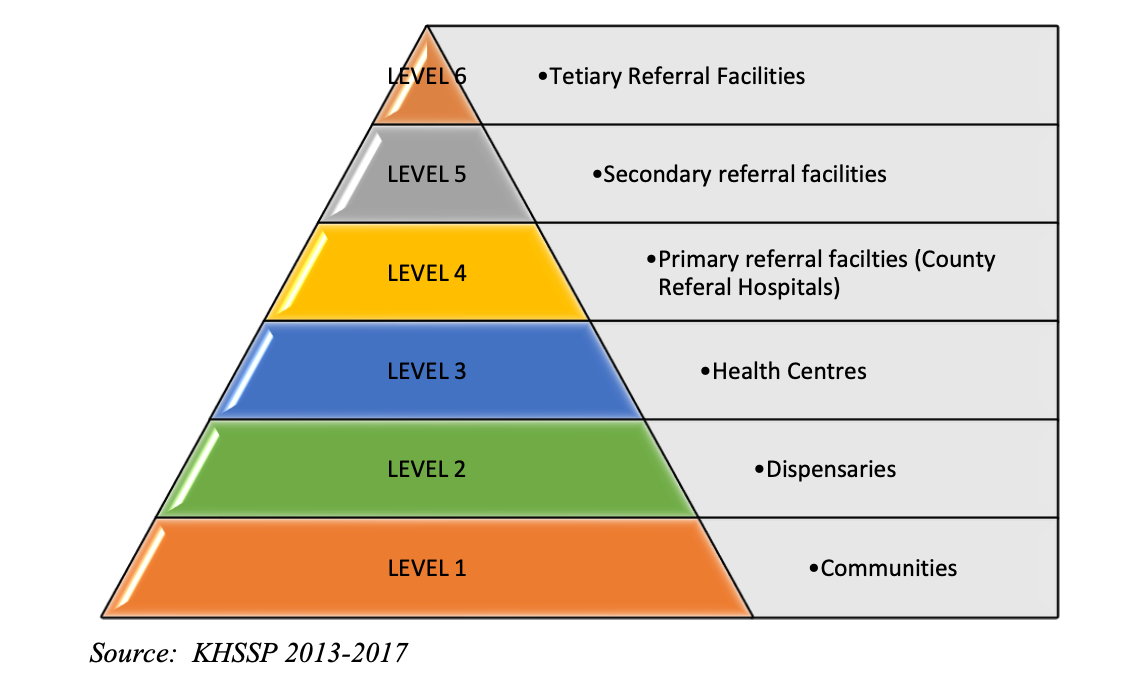
\includegraphics[width=\textwidth]{level of hf.png}
\caption{Kenya Essential Package for Health (KEPH) levels of care}
\label{fig:keph}
\end{figure}


\begin{table}[htbp]
\centering
\caption{Summary statistics of key variables}
 \label{tab:summary}
\begin{tabular}{lrrrrr}
\toprule \toprule
Variable & Mean & SD & Min & Max & N \\
\midrule \midrule
High successful births & 0.28 & 0.45 & 0 & 1 & 462 \\
Internet access is available & 0.29 & 0.45 & 0 & 1 & 1672 \\
Has internet working & 0.97 & 0.17 & 0 & 1 & 477 \\
Rural, urban & 0.16 & 0.37 & 0 & 1 & 1672 \\
Public health facility & 0.73 & 0.44 & 0 & 1 & 1672 \\
Has power interruptions, last 3 months & 0.69 & 0.46 & 0 & 1 & 1477 \\
Has water interruptions, last 3 months & 0.28 & 0.45 & 0 & 1 & 945 \\
Has working refrigerator & 0.94 & 0.24 & 0 & 1 & 1420 \\
Hospitalizes patients & 0.31 & 0.46 & 0 & 1 & 1672 \\
Has blood transfusion & 0.11 & 0.31 & 0 & 1 & 1672 \\
Has c-section & 0.08 & 0.28 & 0 & 1 & 1672 \\
Has diagnostic services & 0.70 & 0.46 & 0 & 1 & 1672 \\
Uses ICT for patient registration & 0.14 & 0.35 & 0 & 1 & 1668 \\
Uses ICT for facility record keeping & 0.17 & 0.37 & 0 & 1 & 1668 \\
Uses ICT for routine comms & 0.34 & 0.47 & 0 & 1 & 1668 \\
Uses ICT for staff training & 0.09 & 0.29 & 0 & 1 & 1668 \\
Uses ICT for clinical consultations & 0.18 & 0.39 & 0 & 1 & 1668 \\
\bottomrule \bottomrule
\end{tabular}
\caption*{\footnotesize Source: 2018 Kenya Service Delivery Indicators survey.}
\end{table}

\begin{table}[htbp]
  \centering
  \caption{Instrumental variable regression results}
  \label{tab:results}
  \begin{tabular}{lc}
    \toprule
    & Successful births\\
    \midrule
    Internet access is available & 0.540***\\
    & (3.51)\\
    Constant & 0.0442\\
    & (0.45)\\
    \midrule
    Observations & 228\\
    Selected instruments & urban, mains power, solar power, cesarean section\\
    First-stage F-statistic & 27.5\\
    \bottomrule
    \multicolumn{2}{l}{\footnotesize{t-statistics in parentheses. * p<0.1, ** p<0.05, *** p<0.01.}}\\
  \end{tabular}
\end{table}



\end{document}

